% ==========================================
% LatexRefinement Step Output: step4-05-19-25-tuesday-all-offset-copy-1-offset-final-copy1.tex
% Model: gemini-3.5-flash
% Temperature: 0.33
% TopP: 0.95
% TopK: 40
% MaxOutputTokens: 65535
% ThinkingBudget: 32765
% ThinkingLevel: HIGH
% Prompt Tokens: 49'827
% Candidates Tokens: 22'525 (inkl. Thinking Tokens)
% Cached Tokens: 0
% Processed on: 2026-07-18 13:18:40
% ==========================================

% ==========================================
% LatexRefinement Step Output: step3-05-19-25-tuesday-all-offset-copy-1-offset-speech_refined-copy1.tex
% Model: gemini-3.5-flash
% Temperature: 0.36
% TopP: 0.95
% TopK: 40
% MaxOutputTokens: 65535
% Processed on: 2026-07-18 13:10:32
% ==========================================

\lecturechapter[13]{Dienstag}{19. Mai}{19. Mai 2026}{Äquivalenzrelationen modulo \texorpdfstring{$n$}{n}, Diffie-Hellman, Chinesischer Restsatz und RSA}
% Old chapter title: Äquivalenzrelationen modulo $n$, Diffie-Hellman und Einheiten in $\mathbb{Z}_n$

\begin{nice-box}[Vorlesungsübersicht \& Kontext]
In dieser Vorlesung setzen wir die Untersuchung der Arithmetik modulo $n$ fort und schlagen die Brücke von der reinen Zahlentheorie zur modernen Kryptographie. Wir behandeln folgende Themen:
\begin{itemize}
    \item \textbf{Äquivalenzrelationen modulo $n$:} Definition der Kongruenz, Restklassen und die Ringstruktur von $\mathbb{Z}_n$.
    \item \textbf{Kryptographische Anwendungen:} Das diskrete Logarithmusproblem und der Diffie-Hellman-Schlüsselaustausch.
    \item \textbf{Einheiten und Körperstruktur:} Charakterisierung invertierbarer Elemente in $\mathbb{Z}_n$ und die Körperstruktur von $\mathbb{Z}_p$.
    \item \textbf{Satz von Lagrange und Euler:} Gruppentheoretische Grundlagen, der Satz von Euler und der Kleine Satz von Fermat.
    \item \textbf{Chinesischer Restsatz \& RSA:} Simultane Kongruenzen, der Ringisomorphismus und das RSA-Kryptosystem.
\end{itemize}
\end{nice-box}

\section{Äquivalenzrelationen modulo \texorpdfstring{$n$}{n}}

\begin{spoken-clean}[00:00:00 - 00:01:57]
Hallo zusammen, wir fangen an. \inlinemetanote{wartet, bis sich die Studierenden beruhigt haben} Wir hatten letzte Woche am Ende noch die Äquivalenzrelationen modulo $n$ gesehen. Das heißt, wir haben gesehen, dass $a$ kongruent zu $b$ modulo $n$ ist ($a \equiv b \pmod n$), falls $n$ ein Teiler von $a - b$ ist ($n \mid (a - b)$). Mit anderen Worten: Wenn wir $a$ und $b$ durch $n$ teilen, erhalten wir denselben Rest. So kann man sich das auch anschauen.

Das heißt, wir schauen uns alle Zahlen an, die denselben Rest ergeben, wenn wir durch $n$ teilen. Gut, und wir haben gesehen, dass das eine Äquivalenzrelation ist. Wenn wir eine Äquivalenzrelation haben, dann gibt uns das Äquivalenzklassen. Das heißt, wir erhalten eine Partition der ganzen Zahlen in ihre Äquivalenzklassen --- wir erhalten also Äquivalenzklassen, und das gibt uns eine Partition von $\mathbb{Z}$.
\end{spoken-clean}

\begin{math-stroke}[Äquivalenzrelation modulo $n$]
\begin{definition}[Äquivalenzrelation modulo $n$]\label[definition]{def:aequiv-mod-n}
Für eine feste natürliche Zahl $n \in \mathbb{N}_{\ge 2}$ definieren wir die Relation der \newterm{Kongruenz modulo $n$} auf den ganzen Zahlen $\mathbb{Z}$ durch:
\begin{equation}\label{eq:aequiv-mod-n}
a \equiv b \pmod n \iff n \mid (a - b).
\end{equation}
Zwei Zahlen $a, b \in \mathbb{Z}$ sind genau dann kongruent modulo $n$, wenn sie bei Division durch $n$ denselben Rest aufweisen.
\end{definition}
\end{math-stroke}

\subsection{Äquivalenzklassen und Partition}

\begin{spoken-clean}[00:01:57 - 00:03:17]
Ich war mir unsicher, wie viel Sie davon bereits gesehen haben. Äquivalenzrelationen haben Sie aber hoffentlich in der Linearen Algebra und/oder der Analysis gesehen. Das ist ein wichtiges Konzept. Es ist wichtig, das gut zu verstehen --- was genau heißt das? Wenn wir eine Äquivalenzrelation haben, dann definiert uns das immer eine Partition der entsprechenden Menge.

Und umgekehrt: Wenn wir eine Partition haben, gibt uns das immer eine Äquivalenzrelation. Sie sehen also, dass das dasselbe ist. Und auch wenn Sie eine Abbildung von einer Menge auf eine andere Menge haben, dann bilden die Fasern eine Partition und somit eine Äquivalenzrelation. Und umgekehrt gibt Ihnen jede Partition respektive Äquivalenzrelation eine Abbildung auf die Äquivalenzklassen.

Einfach um sicher zu sein, dass wir das gut verstanden haben, haben wir das diese Woche nochmals als Übungsaufgabe auf das Übungsblatt gepackt. Wenn Sie also etwas Wichtiges in der Mathematik verstehen wollen, dann lösen Sie bitte diese Übungsaufgabe. Das ist --- auch wenn man es einmal verstanden hat --- gut, wenn man es noch einmal versteht. Ab dem zweiten Jahr nehmen Sie laufend Quotienten bezüglich irgendetwas, und früher oder später werden Sie das auch gut verstehen. Aber wenn Sie es früher gut verstehen, dann haben Sie es nachher einfacher --- zum Beispiel in der Linearen Algebra, wenn Sie die Quotienten von Vektorräumen oder solche Sachen nehmen. Genau.
\end{spoken-clean}

\begin{math-stroke}[Äquivalenzklassen und Partitionen]
Eine Äquivalenzrelation auf einer Menge induziert stets eine Partition dieser Menge in disjunkte Äquivalenzklassen.
\begin{itemize}
    \item \textbf{Äquivalenzklasse:} Für jedes $k \in \mathbb{Z}$ ist die Äquivalenzklasse $[k]$ definiert als die Menge aller zu $k$ kongruenten Elemente:
    \[
    [k] := \{ a \in \mathbb{Z} \mid a \equiv k \pmod n \}.
    \]
    \item \textbf{Partition von $\mathbb{Z}$:} Da jede ganze Zahl bei Division durch $n$ einen eindeutigen Rest $r \in \{0, 1, \dots, n-1\}$ besitzt, zerfällt $\mathbb{Z}$ in genau $n$ disjunkte Äquivalenzklassen:
    \[
    \mathbb{Z} = [0] \;\dot{\cup}\; [1] \;\dot{\cup}\; \dots \;\dot{\cup}\; [n-1].
    \]
\end{itemize}
\end{math-stroke}

\subsection{Quotientenmenge und Quotientenabbildung}

\begin{spoken-clean}[00:03:17 - 00:05:31]
Wir schauen uns jetzt die Äquivalenzklassen an. Das heißt, das ist die Menge aller Zahlen in $\mathbb{Z}$, die äquivalent zu $0$ bezüglich dieser Relation sind --- und das sind genau diejenigen, die durch $n$ teilbar sind. Dann haben wir diejenigen, die äquivalent zu $1$ sind, und das Ganze geht bis $n - 1$. Und das sind schon alle.

Also, hier bei $[k]$ sind das alle Elemente $a \in \mathbb{Z}$, sodass $a$ kongruent zu $k$ modulo $n$ ist. Manchmal schreibt man hier auch noch ein kleines $n$ (z.\,B. $[k]_n$), damit man genau weiß, von welcher Zahl man spricht. Das heißt, davon gibt es jetzt natürlich genau $n$, weil es nur $n$ mögliche Reste gibt, die man haben kann.

Das sind also die Äquivalenzklassen. Und die schreiben wir oft als, sagen wir, $\mathbb{Z}$ modulo $n\mathbb{Z}$ ($\mathbb{Z}/n\mathbb{Z}$). Das ist die Menge der Äquivalenzklassen. Und oft noch einfacher, damit man es etwas leichter schreiben kann, schreibt man das einfach als $\mathbb{Z}_n$ --- mit einem kleinen $n$ hier.

Und das ist ein bisschen verwirrend --- wir machen das jetzt auch so, es ist auch im Skript so ---, aber man darf sich nicht verwirren lassen: In anderen Bereichen der Mathematik, insbesondere in der Zahlentheorie, bezeichnet man mit $\mathbb{Z}_p$, wenn $p$ eine Primzahl ist, die $p$-adischen ganzen Zahlen. Das ist etwas anderes als das hier --- nicht komplett anders, aber doch recht anders. Diese Schreibweise ist also im mathematischen Kontext nicht ganz eindeutig, aber es ist stets klar, was gemeint ist.
\end{spoken-clean}

\begin{math-stroke}[Die Quotientenmenge $\mathbb{Z}_n$]
\begin{definition}[Quotientenmenge / Restklassenring]\label[definition]{def:quotientenmenge-zn}
Die Menge aller Äquivalenzklassen modulo $n$ wird als \newterm{Quotientenmenge} bezeichnet und mit $\mathbb{Z}/n\mathbb{Z}$ oder abkürzend mit $\mathbb{Z}_n$ notiert:
\begin{equation}\label{eq:quotientenmenge-zn}
\mathbb{Z}_n := \mathbb{Z}/n\mathbb{Z} = \{ [0], [1], \dots, [n-1] \}.
\end{equation}
\end{definition}

\begin{notation}[Repräsentanten und Notation]\label[notation]{not:repr-zn}
\begin{itemize}
    \item Für ein Element $a \in \mathbb{Z}$ bezeichnet $[a]$ (oder alternativ $a \pmod n$) die zugehörige Restklasse. Jedes Element $x \in [a]$ heißt \newterm{Repräsentant} dieser Klasse.
    \item \textbf{Warnung zur Notation:} In der fortgeschrittenen Algebra und Zahlentheorie bezeichnet die Notation $\mathbb{Z}_p$ (für eine Primzahl $p$) oft den Ring der $p$-adischen Zahlen. In dieser Vorlesung verwenden wir $\mathbb{Z}_n$ jedoch ausschließlich für den endlichen Restklassenring modulo $n$.
\end{itemize}
\end{notation}
\end{math-stroke}

\subsection{Quotientenabbildung und Operationen}

\begin{spoken-clean}[00:05:31 - 00:07:36]
Wir haben also diese $n$ Elemente in $\mathbb{Z}_n$, der Menge der Äquivalenzklassen. Und wir haben auch die Quotientenabbildung $\pi \colon \mathbb{Z} \to \mathbb{Z}_n$. Diese ordnet jeder Zahl $a$ einfach die Äquivalenzklasse $[a]$ zu. Das ist die Quotientenabbildung.

Gut. Und was wir jetzt tun können, ist, dass wir auf dieser Menge eine Addition und eine Multiplikation definieren. Wir definieren eine Addition und eine Multiplikation auf $\mathbb{Z}_n$ einfach durch $[a] + [b] := [a + b]$. Und ähnlich definieren wir das Produkt $[a] \cdot [b]$ dieser zwei Äquivalenzklassen als die Äquivalenzklasse des Produkts: $[a \cdot b]$.

Und da müssen wir natürlich aufpassen, weil es ja nicht eindeutig ist, welches $a$ hier drin steht --- man könnte ja irgendeinen anderen Repräsentanten nehmen, der äquivalent zu $a$ ist. Da ist a priori nicht klar, dass das wohldefiniert ist. Aber das haben wir letzte Woche noch gesehen: Das hängt gar nicht davon ab, welche Repräsentanten man wählt. Es ergibt am Ende immer dieselbe Äquivalenzklasse. Das heißt, diese Addition und Multiplikation sind wohldefiniert.
\end{spoken-clean}

\begin{math-stroke}[Quotientenabbildung und algebraische Operationen]
\begin{definition}[Quotientenabbildung]\label[definition]{def:quotientenabbildung}
Die kanonische \newterm{Quotientenabbildung} (oder Projektion) $\pi$ ist definiert durch:
\begin{equation}\label{eq:quotientenabbildung}
\pi \colon \mathbb{Z} \to \mathbb{Z}_n, \quad a \mapsto [a].
\end{equation}
\end{definition}

\begin{definition}[Addition und Multiplikation auf $\mathbb{Z}_n$]\label[definition]{def:operationen-zn}
Wir definieren eine Addition und eine Multiplikation auf der Quotientenmenge $\mathbb{Z}_n$ repräsentantenweise durch:
\begin{align}
[a] + [b] &:= [a + b], \label{eq:add-zn} \\
[a] \cdot [b] &:= [a \cdot b]. \label{eq:mul-zn}
\end{align}
\end{definition}

\begin{explanation-of-steps}[Wohldefiniertheit]
Da eine Äquivalenzklasse $[a]$ unendlich viele verschiedene Repräsentanten besitzt, müssen wir sicherstellen, dass die Definitionen \eqref{eq:add-zn} und \eqref{eq:mul-zn} unabhängig von der Wahl der konkreten Repräsentanten $a$ und $b$ sind. Gilt $a \equiv a' \pmod n$ und $b \equiv b' \pmod n$, so muss folgen:
\[
[a + b] = [a' + b'] \quad \text{und} \quad [a \cdot b] = [a' \cdot b'].
\]
Diese fundamentale Eigenschaft wurde in der vergangenen Vorlesung bewiesen.
\end{explanation-of-steps}
\end{math-stroke}

\subsection{Ringstruktur von \texorpdfstring{$\mathbb{Z}_n$}{Zn}}

\begin{spoken-clean}[00:07:36 - 00:09:39]
Wie gesehen --- das war das Lemma der Verträglichkeit der vergangenen Woche (\cref{lem:vertraglichkeit}) --- sind diese Operationen wohldefiniert, d.\,h. sie hängen nicht von der Wahl der Repräsentanten ab. Nun haben wir hier diese Operationen definiert, und wenig erstaunlich lässt sich zeigen, dass $\mathbb{Z}_n$ mit dieser Addition und dieser Multiplikation die Struktur eines Rings besitzt.

Das ist das folgende Lemma: $\mathbb{Z}_n$ mit diesen Operationen ist ein Ring mit den neutralen Elementen $[0]$ und $[1]$. Dabei ist $[0]$ das neutrale Element bezüglich der Addition und $[1]$ das neutrale Element bezüglich der Multiplikation.
\end{spoken-clean}

\begin{math-stroke}[Die Ringstruktur von $\mathbb{Z}_n$]
\begin{lemma}[Ringstruktur von $\mathbb{Z}_n$]\label[lemma]{lem:ringstruktur-zn}
Die Struktur $(\mathbb{Z}_n, +, \cdot, [0], [1])$ bildet einen kommutativen Ring mit Einselement. Dabei gilt:
\begin{itemize}
    \item Das neutrale Element der Addition ist die Restklasse $[0]$.
    \item Das neutrale Element der Multiplikation ist die Restklasse $[1]$.
    \item Das additive Inverse einer Restklasse $[a]$ ist gegeben durch $[-a] = [n - a]$.
\end{itemize}
\end{lemma}
\end{math-stroke}

\subsection{Beweis der Ringeigenschaften}

\begin{spoken-clean}[00:09:39 - 00:13:25]
Gut. Um zu zeigen, dass es sich um einen Ring handelt, muss man natürlich einige Axiome nachprüfen. Das werden wir jetzt nicht alles an die Wandtafel schreiben; ich überlasse es Ihnen, diese alle zu überprüfen. Es folgt aber im Wesentlichen einfach daraus, dass wir bereits wissen, dass $\mathbb{Z}$ ein Ring ist --- also die ganzen Zahlen ein Ring bezüglich Addition und Multiplikation sind.

Per Definition werden alle diese Ringeigenschaften direkt auf $\mathbb{Z}_n$ vererbt. Das liegt daran, dass die Quotientenabbildung $\pi$ surjektiv ist und die Operationen erhält. Wenn $\mathbb{Z}$ ein Ring ist, muss folglich auch $\mathbb{Z}_n$ ein Ring sein. Das ist die grundlegende Idee. Um das mathematisch präzise zu zeigen, muss man natürlich die Axiome einzeln nachprüfen.

Ich schreibe daher an die Tafel: \qt{lässt sich direkt über die entsprechenden Eigenschaften von $\mathbb{Z}$ nachprüfen}. Machen wir einfach ein Beispiel: Wir wollen zeigen, dass die Addition assoziativ ist.

Dazu müssen wir zeigen, dass wenn wir $([a] + [b]) + [c]$ rechnen, dies dasselbe ergibt wie $[a] + ([b] + [c])$. Das ist ganz direkt, denn per Definition ist das die Klasse $[a + b] + [c]$, was wiederum der Klasse $[(a + b) + c]$ entspricht. Da $\mathbb{Z}$ ein Ring ist, wissen wir, dass dies gleich $[a + (b + c)]$ ist --- hier verwenden wir also die Assoziativität in $\mathbb{Z}$. Wenn wir nun rückwärts vorgehen, erhalten wir $[a] + [b + c]$ und somit schließlich $[a] + ([b] + [c])$.
\end{spoken-clean}

\begin{math-stroke}[Beweis der Ringeigenschaften]
\begin{short-proof}[Beweis der Ringeigenschaften von $\mathbb{Z}_n$]
Die Ringaxiome für $\mathbb{Z}_n$ vererben sich direkt von den entsprechenden Eigenschaften des Rings der ganzen Zahlen $(\mathbb{Z}, +, \cdot, 0, 1)$ über die Homomorphieeigenschaft der surjektiven Quotientenabbildung $\pi$.

Exemplarisch weisen wir das \textbf{Assoziativgesetz der Addition} nach. Seien $[a], [b], [c] \in \mathbb{Z}_n$:
\begin{align*}
([a] + [b]) + [c] &= [a + b] + [c] && \text{(per Definition der Addition in $\mathbb{Z}_n$)} \\
&= [(a + b) + c] && \text{(per Definition der Addition in $\mathbb{Z}_n$)} \\
&= [a + (b + c)] && \text{(da die Addition in $\mathbb{Z}$ assoziativ ist)} \\
&= [a] + [b + c] && \text{(Rückrichtung der Definition)} \\
&= [a] + ([b] + [c]) && \text{(Rückrichtung der Definition)}.
\end{align*}
Die übrigen Ringaxiome (Kommutativität, Distributivgesetz, Assoziativität der Multiplikation) lassen sich auf völlig analoge Weise direkt auf die Eigenschaften von $\mathbb{Z}$ zurückführen.
\end{short-proof}
\end{math-stroke}

\section{Kryptographie und Diffie-Hellman-Schlüsselaustausch}

\begin{spoken-clean}[00:13:25 - 00:15:10]
Gut. Auf diese Weise kann man die ganze Liste von Axiomen für alle anderen Ringeigenschaften durchgehen.

Vielleicht machen wir an dieser Stelle einen kleinen Exkurs in die Kryptographie. In der zweiten Hälfte des 20. Jahrhunderts gab es große Errungenschaften dabei, wie man die Zahlentheorie für die Kryptographie nutzen kann --- und zwar unter Verwendung von ganz elementaren Eigenschaften, für die man gar nicht so viel Theorie benötigt. Das erste Verfahren, das ich Ihnen erklären möchte, ist der Diffie-Hellman-Schlüsselaustausch. Das war einer der ersten Proof of Concepts, dass man hier wirklich spannende Dinge tun kann.

Das Problem ist das folgende: In der Kryptographie haben wir üblicherweise Alice, die eine Nachricht an Bob schicken möchte. Die Übermittlung läuft über einen ungesicherten Kanal. Meistens gibt es noch eine dritte Person --- Eve ---, die alles abhört, alles abhören möchte, dies aber eigentlich nicht tun sollte.

Die Frage ist: Wie kann Alice nun eine geheime Nachricht an Bob schicken, ohne dass Eve diese Nachricht versteht? Das ist natürlich ein uraltes Problem, das man schon immer hatte --- bereits bei den Römern und noch viel früher hat man Nachrichten mit Geheimschriften verschlüsselt.
\end{spoken-clean}

\begin{math-stroke}[Kryptographisches Szenario]
\begin{center}
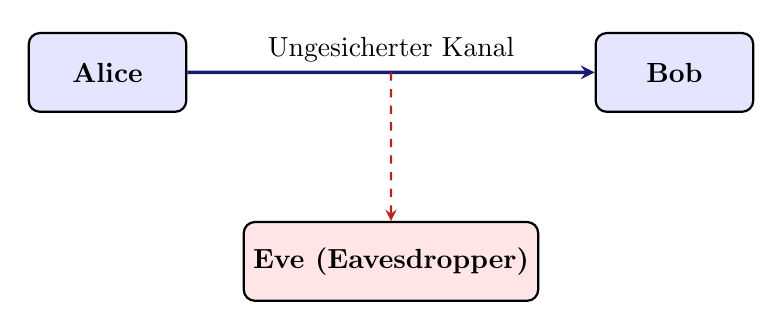
\begin{tikzpicture}[scale=1.2, >=stealth, node distance=2cm]
    % Nodes
    \node[draw, thick, rounded corners, minimum width=2cm, minimum height=1cm, fill=blue!10] (Alice) at (0,2) {\textbf{Alice}};
    \node[draw, thick, rounded corners, minimum width=2cm, minimum height=1cm, fill=blue!10] (Bob) at (6,2) {\textbf{Bob}};
    \node[draw, thick, rounded corners, minimum width=2cm, minimum height=1cm, fill=red!10] (Eve) at (3,0) {\textbf{Eve (Eavesdropper)}};

    % Channel
    \draw[->, very thick, MidnightBlue] (Alice) -- node[midway, above, text=black] {Ungesicherter Kanal} (Bob);
    
    % Eavesdropping paths
    \draw[->, dashed, thick, BrickRed] (3,2) -- (Eve);
\end{tikzpicture}
\end{center}
\end{math-stroke}

\subsection{Das mathematische Problem (Diskreter Logarithmus)}

\begin{spoken-clean}[00:15:10 - 00:18:21]
Was im Informationszeitalter wirklich neu war, ist Folgendes: Für Geheimagenten ist das kein Problem, denn denen gibt man einfach ein Codebuch mit dem geheimen Schlüssel. Das Problem im Alltag ist jedoch, dass die beiden Parteien vorher keinen gemeinsamen Schlüssel austauschen konnten. Wenn Sie beispielsweise im Internet einkaufen und sich ein Buch bei einer Händlerin in New York bestellen, können Sie ihr nicht vorher persönlich einen geheimen Schlüssel vorbeibringen, um Ihre Kreditkartendaten sicher zu übermitteln. Wenn Sie das könnten, bräuchten Sie das Verfahren ja gar nicht erst.

Das Problem ist also, dass man die Vereinbarung komplett in der Öffentlichkeit durchführen muss. Die Frage lautet: Wie können Alice und Bob einen gemeinsamen geheimen Schlüssel vereinbaren? Ein solcher Schlüssel ist mathematisch gesehen einfach eine Zahl.

Das allererste Verfahren in dieser Richtung ist der Diffie-Hellman-\hspace{0pt}Schlüsselaustausch. Was man sich dabei zunutze macht, ist die folgende Asymmetrie --- ein mathematischer Fakt, von dem man überzeugt ist: Es ist sehr einfach, für gegebene Zahlen $a, b > 0$ den Wert $a^b \pmod n$ zu berechnen. Allgemein ist $a^b$ natürlich extrem schwierig zu berechnen, weil die Zahl rasch astronomisch groß wird. Wenn man aber modulo $n$ rechnet, bleibt der Wert immer klein. Zerlegt man den Exponenten $b$ geschickt, kann man das sehr effizient berechnen --- das ist überhaupt kein Problem.
\end{spoken-clean}

\begin{spoken-clean}[00:18:21 - 00:20:33]
Umgekehrt ist es jedoch extrem schwierig, aus dem bekannten Wert $[a^b]$ und der Basis $a$ den Exponenten $b$ wieder herauszufinden. Das dauert rechnerisch sehr lange. Man vermutet zumindest, dass es so ist --- es könnte natürlich sein, dass es einen sehr cleveren Algorithmus gibt, den wir heute noch nicht kennen, um aus den Restklassen $[a^b]$ und $[a]$ das passende $b$ zu bestimmen. Das ist das Problem des diskreten Logarithmus.

Sie können das selbst an einem einfachen Beispiel ausprobieren --- modulo $12$ ist das natürlich sehr übersichtlich: Wenn Sie $3^3 \pmod{12}$ berechnen, sieht man direkt, dass das $3$ ergibt, denn $27 \equiv 3 \pmod{12}$. Wenn ich nun aber umgekehrt frage --- gut, $3$ ist hier ein etwas zu einfaches Beispiel ---, ist es im Kopf extrem schwierig, den diskreten Logarithmus zu ziehen. Der Diffie-Hellman-Schlüsselaustausch macht sich genau diese Asymmetrie zunutze.
\end{spoken-clean}

\begin{math-stroke}[Das diskrete Logarithmusproblem]
\begin{definition}[Einwegfunktion und Diskreter Logarithmus]\label[definition]{def:diskreter-logarithmus}
Das mathematische Fundament vieler asymmetrischer kryptographischer Protokolle basiert auf sogenannten \textbf{Einwegfunktionen} (One-Way Functions):
\begin{enumerate}[label=\textbf{(\arabic*)}]
    \item \textbf{Einfache Richtung (Modulare Exponentiation):} Für gegebenes $a, b, n \in \mathbb{N}$ ist die Berechnung von
    \[
    x \equiv a^b \pmod n
    \]
    äußerst effizient (selbst für sehr große Zahlen mittels des Algorithmus des \emph{Square-and-Multiply}).
    \item \textbf{Schwierige Richtung (Diskretes Logarithmusproblem):} Für vorgegebene Werte $a, x, n \in \mathbb{N}$ ist es rechnerisch extrem aufwendig, den passenden Exponenten $b$ zu bestimmen, sodass gilt:
    \[
    a^b \equiv x \pmod n.
    \]
\end{enumerate}
\end{definition}
\end{math-stroke}

\subsection{Der Diffie-Hellman-Protokollablauf}

\begin{spoken-clean}[00:20:33 - 00:22:40]
Der Diffie-Hellman-Schlüsselaustausch funktioniert wie folgt: Zuerst vereinbaren Alice und Bob öffentlich zwei Zahlen, den Modul $n$ und die Basis $a$. Als Nächstes wählt Alice eine geheime Zahl $r \in \mathbb{N}$ und Bob eine geheime Zahl $s \in \mathbb{N}$.

Nun sendet Alice natürlich nicht ihre geheime Zahl $r$, sondern den berechneten Wert $a^r \pmod n$ an Bob. Analog sendet Bob den Wert $a^s \pmod n$ an Alice.

Das bedeutet: Eve erfährt die Werte $a$, $n$, $a^r$ und $a^s$. Daraus kann sie jedoch weder $r$ noch $s$ effizient ableiten.
\end{spoken-clean}

\begin{spoken-clean}[00:22:40 - 00:25:21]
Im nächsten Schritt berechnet Alice den empfangenen Wert $a^s$ hoch ihre geheime Zahl $r$. Das ergibt in $\mathbb{Z}_n$ die Klasse $[a^{s \cdot r}]$. Bob macht dasselbe mit seinem geheimen $s$: Er berechnet den empfangenen Wert $a^r$ hoch $s$, was ebenfalls $[a^{r \cdot s}]$ ergibt. Das ist nun ihr gemeinsamer geheimer Schlüssel. Genau.

Obwohl dieser gesamte Austausch über einen öffentlichen Kanal stattgefunden hat, besitzen Alice und Bob am Ende eine gemeinsame geheime Zahl, die nur sie beide kennen. Das Ganze beruht auf der Tatsache, dass sich die eine Richtung sehr leicht berechnen lässt, die andere jedoch nicht.

Das ist äußerst elegant und war eine revolutionäre Idee --- obwohl sie mathematisch eigentlich sehr einfach ist. Sie zeigt, dass es möglich ist, über einen ungesicherten Kanal einen gemeinsamen geheimen Schlüssel zu vereinbaren, ohne dass man sich vorher auf irgendetwas geeinigt hat.
\end{spoken-clean}

\begin{math-stroke}[Diffie-Hellman-Schlüsselaustausch]
\textbf{Protokollablauf des Diffie-Hellman-Verfahrens:}
\begin{enumerate}[label=\textbf{(\arabic*)}]
    \item \textbf{Öffentliche Parameter:} Alice und Bob vereinbaren öffentlich eine (große) Modulzahl $n \in \mathbb{N}$ und eine Basis $a \in \mathbb{N}$.
    \item \textbf{Geheime Schlüsselwahl:}
    \begin{itemize}
        \item Alice wählt eine geheime Zahl $r \in \mathbb{N}$.
        \item Bob wählt eine geheime Zahl $s \in \mathbb{N}$.
    \end{itemize}
    \item \textbf{Öffentlicher Austausch:}
    \begin{itemize}
        \item Alice berechnet $[a^r] \in \mathbb{Z}_n$ und sendet diesen Wert an Bob.
        \item Bob berechnet $[a^s] \in \mathbb{Z}_n$ und sendet diesen Wert an Alice.
    \end{itemize}
    \item \textbf{Schlüsselberechnung:}
    \begin{itemize}
        \item Alice berechnet $[a^s]^r = [a^{s \cdot r}] \in \mathbb{Z}_n$.
        \item Bob berechnet $[a^r]^s = [a^{r \cdot s}] \in \mathbb{Z}_n$.
    \end{itemize}
    \begin{explanation-of-steps}[Potenzgesetze in $\mathbb{Z}_n$]
    Streng genommen verwenden wir hier implizit, dass die Potenzgesetze (wie $(a^r)^s = a^{r \cdot s}$) auch beim Rechnen mit Restklassen erhalten bleiben. Da die Multiplikation in $\mathbb{Z}_n$ wohldefiniert ist, folgt dies durch iterierte Anwendung der Eigenschaft $[x] \cdot [y] = [x \cdot y]$.
    \end{explanation-of-steps}
\end{enumerate}
Da $s \cdot r = r \cdot s$ in $\mathbb{Z}$ gilt, erhalten beide Parteien dieselbe Restklasse:
\begin{equation}\label{eq:dh-schluessel}
K := [a^{r \cdot s}] \in \mathbb{Z}_n.
\end{equation}
Dieser Wert $K$ dient fortan als gemeinsamer geheimer Schlüssel. Ein Angreifer (Eve), der lediglich $n, a, [a^r]$ und $[a^s]$ belauscht, kann ohne Lösung des diskreten Logarithmusproblems nicht auf $r$ oder $s$ und somit nicht auf $K$ schließen.
\end{math-stroke}

\section{Einheiten und Körperstruktur in \texorpdfstring{$\mathbb{Z}_n$}{Zn}}

\begin{spoken-clean}[00:25:21 - 00:27:46]
Nun aber, wieder zurück zur Theorie. Wir haben gesehen, dass diese $\mathbb{Z}_n$ Ringe sind. In Ringen gibt es Elemente, die ein multiplikatives Inverses besitzen, und andere, bei denen das nicht der Fall ist. Wenn es ein Körper ist, hat jedes Element außer der Null ein multiplikatives Inverses; in allgemeinen Ringen muss das jedoch nicht so sein.

Die Frage lautet nun: Welche Elemente besitzen ein multiplikatives Inverses? Betrachten wir als Beispiel $\mathbb{Z}_{12}$: Die Klasse $[0]$ hat natürlich kein Inverses, aber auch $[2]$ hat kein multiplikatives Inverses. Sie finden kein Element $[a] \in \mathbb{Z}_{12}$, sodass $2 \cdot a \equiv 1 \pmod{12}$ gilt. Das geht nicht, denn die Vielfachen von $2$ modulo $12$ sind $2, 4, 6, 8, 10, 0$ --- bevor Sie also bei der $1$ ankommen, landen Sie wieder bei der $0$, und das Ganze beginnt von vorn.

Hingegen funktioniert es für $[5]$ sehr wohl, denn $5 \cdot 5 = 25 \equiv 1 \pmod{12}$. Somit besitzt $[5]$ ein multiplikatives Inverses.

Die nächste Proposition formalisiert diese Beobachtung. Proposition: Sei $n \ge 2$ und $[a] \in \mathbb{Z}_n$. Es existiert ein $[b] \in \mathbb{Z}_n$ mit $[a] \cdot [b] = [1]$ genau dann, wenn $\operatorname{ggT}(a, n) = 1$ gilt --- also genau dann, wenn die beiden Zahlen teilerfremd sind. Das erklärt, warum es für $[5]$ modulo $12$ klappt, für $[2]$ modulo $12$ hingegen nicht.
\end{spoken-clean}

\begin{math-stroke}[Invertierbarkeit in $\mathbb{Z}_n$]
\begin{proposition}[Multiplikatives Inverses in $\mathbb{Z}_n$]\label[proposition]{prop:inverses-zn}
Sei $n \in \mathbb{N}_{\ge 2}$ und $[a] \in \mathbb{Z}_n$. Die Restklasse $[a]$ besitzt genau dann ein multiplikatives Inverses $[b] \in \mathbb{Z}_n$ mit
\begin{equation}\label{eq:inverses-zn}
[a] \cdot [b] = [1],
\end{equation}
wenn $a$ und $n$ teilerfremd sind, d.\,h. wenn gilt:
\[
\operatorname{ggT}(a, n) = 1.
\]
\end{proposition}
\end{math-stroke}

\subsection{Beweis der Invertierbarkeit}

\begin{spoken-clean}[00:27:46 - 00:29:06]
Sei $d$ der größte gemeinsame Teiler. Das heißt, $d$ teilt sowohl $a$ als auch $n$. Somit folgt, dass $d$ auch $a \cdot b - k \cdot n$ teilt. Das ist aber nach Voraussetzung genau $1$. Das bedeutet, $d$ ist ein Teiler von $1$, und da $d$ eine natürliche Zahl ist, folgt $d = 1$. Das beweist die eine Richtung.

Falls umgekehrt $\operatorname{ggT}(a, n) = 1$ gilt, wissen wir aus der vergangenen Woche, dass ganze Zahlen $b, \ell \in \mathbb{Z}$ existieren, sodass $a \cdot b + n \cdot \ell = 1$ gilt. Das war der Satz von Bézout (\cref{prop:ggt-bezout}), den wir bewiesen haben: Wir finden stets ganze Zahlen $b$ und $\ell$, sodass diese Linearkombination gleich dem größten gemeinsamen Teiler ist.
\end{spoken-clean}

\begin{spoken-clean}[00:29:06 - 00:30:56]
Das bedeutet aber direkt, dass $a \cdot b = -\ell \cdot n + 1$ gilt, woraus $a \cdot b \equiv 1 \pmod n$ folgt. Somit ist nach Definition $[a] \cdot [b] = [1]$. Wir verstehen die invertierbaren Elemente in diesen Ringen also nun sehr gut.

Ein direktes Korollar daraus lautet: Der Restklassenring $\mathbb{Z}_n$ ist genau dann ein Körper, wenn $n$ eine Primzahl ist.

Der Beweis folgt unmittelbar aus der Proposition: Wir wissen, dass $\mathbb{Z}_n$ genau dann ein Körper ist, wenn für jede Klasse $[a] \neq [0]$ gilt, dass $[a]$ invertierbar ist.
\end{spoken-clean}

\begin{math-stroke}[Beweis der Invertierbarkeit]
\begin{short-proof}[Beweis von Proposition \ref{prop:inverses-zn}]
Sei $d := \operatorname{ggT}(a, n)$.

\textbf{Richtung $(\implies)$:}
Angenommen, $[a]$ ist invertierbar in $\mathbb{Z}_n$. Dann existiert ein $[b] \in \mathbb{Z}_n$ mit $[a] \cdot [b] = [1]$. Nach Definition der Multiplikation bedeutet dies:
\[
a \cdot b \equiv 1 \pmod n \implies a \cdot b - k \cdot n = 1 \quad \text{für ein } k \in \mathbb{Z}.
\]
Da $d = \operatorname{ggT}(a, n)$ gilt, teilt $d$ sowohl $a$ als auch $n$. Folglich teilt $d$ auch jede ganzzahlige Linearkombination dieser Zahlen:
\[
d \mid (a \cdot b - k \cdot n) \implies d \mid 1.
\]
Da $d \in \mathbb{N}_{>0}$, folgt zwingend $d = 1$.

\textbf{Richtung $(\impliedby)$:}
Angenommen, $\operatorname{ggT}(a, n) = 1$. Nach dem Lemma von Bézout (\cref{prop:ggt-bezout}) existieren ganze Zahlen $b, \ell \in \mathbb{Z}$, sodass gilt:
\[
a \cdot b + n \cdot \ell = 1 \implies a \cdot b = -\ell \cdot n + 1 \implies a \cdot b \equiv 1 \pmod n.
\]
Gehen wir zu den Restklassen über, so folgt nach Definition der Multiplikation in $\mathbb{Z}_n$:
\[
[a \cdot b] = [1] \implies [a] \cdot [b] = [1].
\]
Somit ist $[b] \in \mathbb{Z}_n$ das gesuchte multiplikative Inverse von $[a]$.
\end{short-proof}
\end{math-stroke}

\subsection{Körperstruktur von \texorpdfstring{$\mathbb{Z}_n$}{Zn}}

\begin{spoken-clean}[00:30:56 - 00:33:13]
Genau. Wenn $n$ eine Primzahl ist, dann sind alle Zahlen zwischen $1$ und $n-1$ teilerfremd zu $n$. Somit besitzt jede Restklasse außer der Nullklasse ein multiplikatives Inverses. Das macht $\mathbb{Z}_n$ zu einem Körper, den wir oft auch als $\mathbb{F}_p$ schreiben, wenn $n = p$ eine Primzahl ist. Das ist eine fundamentale Struktur in der Algebra und Zahlentheorie. Lassen Sie uns das an der Tafel festhalten. Wir definieren nun ganz allgemein den Begriff der Einheit in einem Ring, um diese invertierbaren Elemente systematisch zu untersuchen.
\end{spoken-clean}

\begin{math-stroke}[Körperstruktur von $\mathbb{Z}_n$]
\begin{corollary}[Körperstruktur von $\mathbb{Z}_n$]\label[corollary]{cor:koerper-zn}
Der Restklassenring $(\mathbb{Z}_n, +, \cdot, [0], [1])$ ist genau dann ein Körper, wenn $n$ eine Primzahl ist.
\end{corollary}

\begin{short-proof}[Beweis des Korollars \ref{cor:koerper-zn}]
Ein kommutativer Ring mit Einselement $[1] \neq [0]$ ist ein Körper genau dann, wenn jedes von Null verschiedene Element ein multiplikatives Inverses besitzt. Es gilt:
\begin{align*}
\mathbb{Z}_n \text{ ist ein Körper} &\iff \forall [a] \in \mathbb{Z}_n \setminus \{[0]\} \colon [a] \text{ ist invertierbar} \\
&\iff \forall a \in \{1, 2, \dots, n-1\} \colon \operatorname{ggT}(a, n) = 1 \\
&\iff n \text{ besitzt keine echten Teiler} \\
&\iff n \text{ ist eine Primzahl}.
\end{align*}
Dies beweist das Korollar.
\end{short-proof}
\end{math-stroke}

\section{Die Einheitengruppe \texorpdfstring{$\mathbb{Z}_n^*$}{Zn*}}

\begin{spoken-clean}[00:33:13 - 00:36:01]
Wir definieren die menge $\mathbb{Z}_n^*$ als die Menge aller Einheiten in $\mathbb{Z}_n$. Das sind genau die Restklassen, die teilerfremd zu $n$ sind, wie wir gerade bewiesen haben. Wir können diese Menge als eine Gruppe bezüglich der Multiplikation betrachten. Warum bildet sie eine Gruppe? Nun, das neutrale Element ist die Klasse $[1]$, die natürlich enthalten ist, da $1 \cdot 1 = 1$ gilt. Wenn wir zwei Einheiten $[a]$ und $[b]$ haben, ist auch ihr Produkt wieder eine Einheit, da das Inverse von $[a] \cdot [b]$ einfach das Produkt der Inversen ist, also $[b]^{-1} \cdot [a]^{-1}$. Das heißt, die Multiplikation ist auf dieser Menge abgeschlossen. Die Assoziativität vererbt sich direkt vom Ring, und jedes Element besitzt per Definition ein Inverses in dieser Menge. Es handelt sich also tatsächlich um eine Gruppe --- wir nennen sie die Einheitengruppe von $\mathbb{Z}_n$.
\end{spoken-clean}

\begin{math-stroke}[Definition der Einheiten]
\begin{definition}[Einheit und Einheitengruppe]\label[definition]{def:einheit-zn}
Ein Element $[a] \in \mathbb{Z}_n$ heißt eine \newterm{Einheit}, falls ein multiplikatives Inverses $[b] \in \mathbb{Z}_n$ existiert, sodass gilt:
\begin{equation}\label{eq:einheit-def}
[a] \cdot [b] = [1].
\end{equation}
Die Menge aller Einheiten in $\mathbb{Z}_n$ wird mit $\mathbb{Z}_n^*$ (oder alternativ mit $\mathbb{Z}_n^\times$) bezeichnet:
\begin{equation}\label{eq:einheitengruppe-def}
\mathbb{Z}_n^* := \{ [a] \in \mathbb{Z}_n \mid [a] \text{ ist eine Einheit} \}.
\end{equation}
\end{definition}

\begin{remark}[Charakterisierung der Einheiten]
Nach Proposition \ref{prop:inverses-zn} besteht die Einheitengruppe $\mathbb{Z}_n^*$ genau aus denjenigen Restklassen, deren Repräsentanten teilerfremd zum Modul $n$ sind:
\[
\mathbb{Z}_n^* = \{ [a] \in \mathbb{Z}_n \mid \operatorname{ggT}(a, n) = 1 \;. \}
\]
\end{remark}
\end{math-stroke}

\subsection{Gruppenstruktur der Einheiten}

\begin{math-stroke}[Gruppenstruktur der Einheiten]
\begin{proposition}[Die Einheitengruppe $(\mathbb{Z}_n^*, \cdot)$]\label[proposition]{prop:einheiten-gruppe}
Die Menge der Einheiten $\mathbb{Z}_n^*$ bildet bezüglich der Multiplikation eine kommutative (abelsche) Gruppe.
\end{proposition}

\begin{short-proof}
Wir verifizieren die Gruppenaxiome für $(\mathbb{Z}_n^*, \cdot)$:
\begin{enumerate}[label=\textbf{(\arabic*)}]
    \item \textbf{Abgeschlossenheit:} Seien $[a], [a'] \in \mathbb{Z}_n^*$. Dann existieren $[b], [b'] \in \mathbb{Z}_n$ mit $[a] \cdot [b] = [1]$ und $[a'] \cdot [b'] = [1]$. Für das Produkt gilt:
    \[
    ([a] \cdot [a']) \cdot ([b'] \cdot [b]) = ([a] \cdot [b]) \cdot ([a'] \cdot [b']) = [1] \cdot [1] = [1].
    \]
    Da $[b'] \cdot [b] \in \mathbb{Z}_n$, ist auch $[a] \cdot [a']$ invertierbar, folglich gilt $[a] \cdot [a'] \in \mathbb{Z}_n^*$.
    \item \textbf{Assoziativität:} Folgt direkt aus der Assoziativität der Multiplikation im Ring $\mathbb{Z}_n$.
    \item \textbf{Neutrales Element:} Es gilt $[1] \cdot [1] = [1]$, somit ist $[1] \in \mathbb{Z}_n^*$ das neutrale Element.
    \item \textbf{Inverses Element:} Für jedes $[a] \in \mathbb{Z}_n^*$ existiert per Definition ein $[b] \in \mathbb{Z}_n$ mit $[a] \cdot [b] = [1]$. Da diese Gleichung symmetrisch ist, ist auch $[b]$ eine Einheit, also $[b] \in \mathbb{Z}_n^*$, und es gilt $[a]^{-1} = [b]$.
\end{enumerate}
Da die Multiplikation in $\mathbb{Z}_n$ kommutativ ist, ist $(\mathbb{Z}_n^*, \cdot)$ eine abelsche Gruppe.
\end{short-proof}
\end{math-stroke}

\subsection{Die Eulersche \texorpdfstring{$\varphi$}{phi}-Funktion}

\begin{spoken-clean}[00:36:01 - 00:38:56]
Wie groß ist nun diese Gruppe? Die Ordnung dieser Gruppe --- also die Anzahl der Elemente in $\mathbb{Z}_n^*$ --- wird durch eine sehr berühmte Funktion der Zahlentheorie beschrieben: die eulersche $\varphi$-Funktion. Wir schreiben dafür das griechische $\varphi(n)$. Das ist per Definition genau die Anzahl der Zahlen im Intervall $[1, n]$, die teilerfremd zu $n$ sind. Das heißt, wir können schreiben: Die Mächtigkeit von $\mathbb{Z}_n^*$ ist genau $\varphi(n)$. Wenn $p$ eine Primzahl ist, ist das besonders einfach, da alle Zahlen von $1$ bis $p-1$ teilerfremd zu $p$ sind. Für eine Primzahl $p$ gilt folglich immer $\varphi(p) = p - 1$. Das ist ein sehr schönes Ergebnis, das wir im Folgenden oft verwenden werden.
\end{spoken-clean}

\begin{math-stroke}[Eulersche $\varphi$-Funktion]
\begin{definition}[Eulersche $\varphi$-Funktion]\label[definition]{def:euler-phi-w13}
Die \newterm{Eulersche $\varphi$-Funktion} $\varphi \colon \mathbb{N}_{>0} \to \mathbb{N}$ ordnet jeder natürlichen Zahl $n$ die Anzahl aller zu $n$ teilerfremden natürlichen Zahlen im Intervall $[1, n]$ zu:
\begin{equation}\label{eq:euler-phi}
\varphi(n) := |\{ k \in \mathbb{N} \mid 1 \le k \le n \text{ und } \operatorname{ggT}(k, n) = 1 \}|.
\end{equation}
Es gilt somit für die Ordnung der Einheitengruppe:
\begin{equation}\label{eq:ordnung-einheitengruppe}
|\mathbb{Z}_n^*| = \varphi(n).
\end{equation}
\end{definition}

\begin{example}[Eulersche $\varphi$-Funktion für Primzahlen]\label[example]{ex:phi-primzahl}
Ist $p$ eine Primzahl, so ist jede Zahl $k \in \{1, \dots, p-1\}$ teilerfremd zu $p$. Es gilt daher:
\begin{equation}\label{eq:phi-primzahl}
\varphi(p) = p - 1.
\end{equation}
\end{example}
\end{math-stroke}

\section{Der Satz von Lagrange für abelsche Gruppen}

\begin{spoken-clean}[00:38:56 - 00:41:36]
Das ist also die eulersche $\varphi$-Funktion. Jetzt wollen wir einen sehr allgemeinen und fundamentalen Satz aus der Gruppentheorie beweisen, der uns erlaubt, diese Einheitenstruktur noch viel tiefer zu verstehen. Es handelt sich um den Satz von Lagrange für abelsche Gruppen bzw. eine direkte Konsequenz daraus. Der Satz besagt: Wenn wir eine endliche abelsche Gruppe $G$ mit dem neutralen Element $e$ haben, dann gilt für jedes Element $g \in G$, dass $g^{|G|} = e$ ist --- wenn wir also $g$ hoch die Gruppenordnung nehmen, erhalten wir genau das neutrale Element $e$. Das ist ein wunderschöner Satz, und der Beweis ist erstaunlich elegant. Wir definieren dafür eine Abbildung, die jedes Element mit $g$ multipliziert, und nutzen aus, dass diese Abbildung eine Bijektion ist. Lassen Sie uns das an der Tafel aufschreiben.
\end{spoken-clean}

\begin{math-stroke}[Satz von Lagrange für abelsche Gruppen]
\begin{theorem}[Satz von Lagrange für endliche abelsche Gruppen]\label[theorem]{thm:lagrange-abelsch}
Sei $(G, \cdot, e)$ eine endliche abelsche Gruppe mit neutralem Element $e$. Für jedes Element $g \in G$ gilt:
\begin{equation}\label{eq:lagrange-abelsch}
g^{|G|} = e.
\end{equation}
\end{theorem}
\end{math-stroke}

\subsection{Beweis des Satzes von Lagrange}

\begin{spoken-clean}[00:41:36 - 00:44:16]
Der Beweis verläuft wie folgt: Wir betrachten die Abbildung $\psi \colon G \to G$, die jedes Element $h$ auf $g \cdot h$ abbildet. Da $G$ eine Gruppe ist, besitzt jedes Element ein Inverses, und wir können leicht zeigen, dass diese Abbildung bijektiv ist. Sie ist injektiv, denn aus $g \cdot h_1 = g \cdot h_2$ folgt durch Multiplikation von links mit $g^{-1}$ direkt $h_1 = h_2$. Und sie ist surjektiv, weil für jedes $y \in G$ das Element $g^{-1} \cdot y$ ein gültiges Urbild darstellt.

Da diese Abbildung eine Bijektion ist, permutiert sie einfach die Elemente der Gruppe. Das bedeutet: Wenn wir das Produkt über alle Elemente der Gruppe bilden, ist das Produkt über alle $h \in G$ genau dasselbe wie das Produkt über alle $g \cdot h$ in $G$. Da die Gruppe abelsch ist, können wir die Faktoren beliebig umordnen. Wir können also das $g$ aus jedem Faktor herausziehen. Da es genau $|G|$ viele Elemente gibt, erhalten wir $g^{|G|}$ mal das Produkt über alle $h$. Da wir in einer Gruppe arbeiten, können wir dieses Produkt auf beiden Seiten kürzen und erhalten genau $g^{|G|} = e$. Das ist wirklich ein extrem eleganter Beweis! (Dieser sogenannte Permutationstrick nutzt genial die Invarianz des Gesamtprodukts unter Gruppen-Translationen aus.)
\end{spoken-clean}

\begin{math-stroke}[Beweis des Satzes von Lagrange]
\begin{short-proof}[Beweis von Theorem \ref{thm:lagrange-abelsch}]
Wir definieren für ein festes Element $g \in G$ die Abbildung:
\[
\psi \colon G \to G, \quad h \mapsto g \cdot h.
\]
Diese Abbildung ist bijektiv:
\begin{itemize}
    \item \textbf{Injektivität:} Für $h_1, h_2 \in G$ gilt:
    \[
    \psi(h_1) = \psi(h_2) \implies g \cdot h_1 = g \cdot h_2 \implies g^{-1} \cdot (g \cdot h_1) = g^{-1} \cdot (g \cdot h_2) \implies h_1 = h_2.
    \]
    \item \textbf{Surjektivität:} Für jedes $y \in G$ existiert das Urbild $h := g^{-1} \cdot y \in G$, da gilt:
    \[
    \psi(g^{-1} \cdot y) = g \cdot (g^{-1} \cdot y) = y.
    \]
\end{itemize}
Da $\psi$ eine Bijektion auf der endlichen Menge $G$ ist, gilt für das Produkt aller Gruppenelemente:
\[
\prod_{h \in G} h = \prod_{h \in G} \psi(h) = \prod_{h \in G} (g \cdot h).
\]
Da die Gruppe $G$ abelsch (kommutativ) ist, können wir das rechte Produkt umordnen und erhalten:
\[
\prod_{h \in G} (g \cdot h) = \left( \prod_{h \in G} g \right) \cdot \left( \prod_{h \in G} h \right) = g^{|G|} \cdot \prod_{h \in G} h.
\]
Gleichsetzen der beiden Ausdrücke liefert:
\[
\prod_{h \in G} h = g^{|G|} \cdot \prod_{h \in G} h.
\]
Da $G$ eine Gruppe ist, besitzt das Produkt $\prod_{h \in G} h$ ein multiplikatives Inverses in $G$. Multiplikation mit diesem Inversen liefert das gewünschte Resultat:
\[
e = g^{|G|}.
\]
\end{short-proof}
\end{math-stroke}

\section{Der Satz von Euler und der Kleine Satz von Fermat}

\begin{spoken-clean}[00:44:16 - 00:46:56]
Das ist ein fantastisches Ergebnis! Und jetzt können wir dieses allgemeine gruppentheoretische Resultat direkt auf unsere Einheitengruppe $\mathbb{Z}_n^*$ anwenden. Da $\mathbb{Z}_n^*$ eine endliche abelsche Gruppe der Ordnung $\varphi(n)$ ist, erhalten wir sofort, dass für jede Einheit $[a] \in \mathbb{Z}_n^*$ gilt: $[a]^{\varphi(n)} = [1]$. Das ist der berühmte Satz von Euler!

Wenn wir den Spezialfall betrachten, dass $n = p$ eine Primzahl ist, gilt $\varphi(p) = p - 1$. Für jede Zahl $a$, die kein Vielfaches von $p$ ist, gilt also: $a^{p-1} \equiv 1 \pmod p$. Das ist der Kleine Satz von Fermat! Es ist eines der ältesten und wichtigsten Resultate der Zahlentheorie, das wir hier als einfaches Korollar eines allgemeinen gruppentheoretischen Prinzips geschenkt bekommen. Das zeigt die enorme Kraft der Abstraktion in der modernen Algebra.
\end{spoken-clean}

\subsection{Der Satz von Euler}
\begin{math-stroke}
\begin{theorem}[Satz von Euler]\label[theorem]{thm:satz-von-euler}
Sei $n \in \mathbb{N}_{\ge 2}$ und $a \in \mathbb{Z}$ mit $\operatorname{ggT}(a, n) = 1$. Dann gilt:
\begin{equation}\label{eq:satz-von-euler}
a^{\varphi(n)} \equiv 1 \pmod n.
\end{equation}
\end{theorem}

\begin{short-proof}
Da $\operatorname{ggT}(a, n) = 1$, ist die Restklasse $[a]$ ein Element der endlichen abelschen Einheitengruppe $\mathbb{Z}_n^*$. Die Ordnung dieser Gruppe ist $|\mathbb{Z}_n^*| = \varphi(n)$ (\cref{def:euler-phi}). Die Anwendung von Theorem \ref{thm:lagrange-abelsch} auf die Gruppe $G = \mathbb{Z}_n^*$ liefert direkt:
\[
[a]^{|\mathbb{Z}_n^*|} = [1] \implies [a]^{\varphi(n)} = [1].
\]
Nach Definition der Multiplikation in $\mathbb{Z}_n$ entspricht dies der Kongruenz:
\[
a^{\varphi(n)} \equiv 1 \pmod n.
\]
Dies beweist den Satz.
\end{short-proof}
\end{math-stroke}

\subsection{Der Kleine Satz von Fermat}

\begin{spoken-clean}[00:46:56 - 00:49:26]
Lassen Sie uns das auch für den Kleinen Satz von Fermat explizit aufschreiben. Wie gesagt, das ist einfach der Spezialfall für Primzahlen. Wenn $p$ prim ist, dann ist jede Zahl $a$, die kein Vielfaches von $p$ ist, teilerfremd zu $p$. Das heißt, $\operatorname{ggT}(a, p) = 1$. Da $\varphi(p) = p-1$ ist, folgt die Behauptung sofort. Ich schreibe das an die Tafel. Danach möchte ich Ihnen ein bisschen etwas über Pierre de Fermat erzählen, der diesen Satz im 17. Jahrhundert formuliert hat. Er war ein faszinierender Charakter --- eigentlich kein Berufsmathematiker, sondern Jurist und Parlamentsrat in Toulouse ---, aber er hat die Zahlentheorie seiner Zeit maßgeblich geprägt.
\end{spoken-clean}

\begin{math-stroke}[Der Kleine Satz von Fermat]
\begin{corollary}[Kleiner Satz von Fermat]\label[corollary]{cor:kleiner-fermat}
Sei $p$ eine Primzahl und $a \in \mathbb{Z}$ mit $p \nmid a$. Dann gilt:
\begin{equation}\label{eq:kleiner-fermat}
a^{p-1} \equiv 1 \pmod p.
\end{equation}
\end{corollary}

\begin{short-proof}
Da $p$ eine Primzahl ist und $p \nmid a$ gilt, ist $\operatorname{ggT}(a, p) = 1$. Nach dem Satz von Euler (\cref{thm:satz-von-euler}) gilt:
\[
a^{\varphi(p)} \equiv 1 \pmod p.
\]
Da für Primzahlen $\varphi(p) = p-1$ gilt (\cref{ex:phi-primzahl}), folgt durch Einsetzen sofort:
\[
a^{p-1} \equiv 1 \pmod p.
\]
Dies beweist das Korollar.
\end{short-proof}
\end{math-stroke}

\section{Historischer Exkurs: Pierre de Fermat}

\begin{spoken-clean}[00:49:26 - 00:51:56]
Ich habe hier ein paar Folien vorbereitet. \inlinemetanote{schaltet den Projektor ein und zeigt ein Porträt von Pierre de Fermat} Pierre de Fermat hat von 1601 bis 1665 gelebt. Er war, wie gesagt, Parlamentsrat in Toulouse und hat die Mathematik nur als Hobby betrieben, allerdings auf einem unglaublich hohen Niveau. Er hat fast keinen seiner Beweise veröffentlicht, sondern seine Resultate oft in Briefen an Freunde wie Blaise Pascal oder Marin Mersenne mitgeteilt oder einfach als Randnotizen in seinen Büchern aufgeschrieben.

Das berühmteste Beispiel dafür ist sicherlich der Große Satz von Fermat, auch Fermats Letzter Satz genannt. Er hat in seinem Exemplar der \emph{Arithmetica} von Diophant an den Rand geschrieben, dass er einen wahrhaft wunderbaren Beweis dafür gefunden habe, dass die Gleichung $x^n + y^n = z^n$ für $n \ge 3$ keine ganzzahligen Lösungen außer der trivialen Nulllösung besitzt --- aber der Rand des Buches sei zu schmal, um den Beweis aufzunehmen.
\end{spoken-clean}

\begin{meta-note}[Projizierter Inhalt: Porträt von Pierre de Fermat]
Der Projektor zeigt ein historisches Porträt von Pierre de Fermat mit den Lebensdaten:
\[
\text{Pierre de Fermat, 1601 -- 1655}
\]
\emph{Hinweis zur Jahreszahl:} Auf der Folie ist fälschlicherweise das Todesjahr $1655$ angegeben; historisch korrekt verstarb Fermat im Jahr $1665$.
\end{meta-note}

\begin{spoken-clean}[00:51:56 - 00:54:26]
Diese Randnotiz hat die mathematische Welt über 300 Jahre lang in Atem gehalten! Generationen von Mathematikerinnen und Mathematikern haben versucht, diesen Satz zu beweisen. Er wurde erst 1995 von Andrew Wiles und Richard Taylor mit extrem modernen Methoden der algebraischen Geometrie und der Modulformen bewiesen. Man ist sich heute ziemlich sicher, dass Fermat selbst keinen korrekten Beweis hatte, weil die dafür benötigte Mathematik im 17. Jahrhundert schlicht noch nicht existierte.

Aber diese Suche nach dem Beweis war der Motor für die Entwicklung der gesamten modernen algebraischen Zahlentheorie! Eine sehr wichtige Rolle spielte dabei auch Sophie Germain im frühen 19. Jahrhundert --- eine französische Mathematikerin, die unter einem männlichen Pseudonym arbeitete und bedeutende Fortschritte für eine große Klasse von Primzahlen erzielte. Morgen gibt es übrigens einen sehr spannenden Vortrag zu Sophie Germain und ihrer Mathematik hier an der Universität, zu dem Sie alle herzlich eingeladen sind.
\end{spoken-clean}

\subsection{Fermats Letzter Satz}

\begin{spoken-clean}[00:55:32 - 00:57:02]
Das war über 300 Jahre lang sozusagen der Motor für die Zahlentheorie --- es wurde enorm viel interessante Mathematik entwickelt, nur um diese Vermutung zu beweisen. Es ist immer gut für ein Gebiet, wenn es so inspirierende, starke, offene Probleme gibt. Das wirkt wie ein Zugpferd: Wenn es einen großen Stern am Himmel gibt, den man erreichen möchte, hilft das, die Strukturen im Allgemeinen besser zu verstehen. Man kann darüber natürlich noch viel erzählen.

Jedenfalls wurde es in den 90er Jahren schlussendlich bewiesen. Viele von Ihnen kennen vielleicht das Buch von Simon Singh zu diesem Thema --- auf Deutsch \qt{Fermats letzter Satz}, auf Englisch \qt{Fermat's Last Theorem}. Das ist ein sehr schönes Buch und absolut empfehlenswert: sehr einfach zu lesen, populärwissenschaftlich geschrieben, aber extrem spannend.

Es erzählt \inlinemetanote{wischt die Tafel} die Geschichte dieses Satzes, was auch ein Stück weit die Geschichte der Mathematik selbst ist. Es liest sich sehr flüssig und ist dennoch sehr informativ. Ich empfehle es auch immer gerne Nicht-Mathematikern, wenn sie verstehen wollen, warum Menschen so gerne Mathematik betreiben.
\end{spoken-clean}

\begin{spoken-clean}[00:57:02 - 00:58:11]
Das nur als eine kleine Seitenbemerkung, aber es ist ein wichtiges Resultat und vor allem ein bedeutendes Stück Mathematikgeschichte, das Sie alle einmal gehört haben sollten.

Übrigens hat auch Sophie Germain --- eine hervorragende Mathematikerin des späten 18. und frühen 19. Jahrhunderts --- wesentlich zur Lösung des Fermatschen Satzes beigetragen. Morgen gibt es, wie gesagt, einen Vortrag dazu hier an der Universität, zu dem Sie herzlich eingeladen sind.
\end{spoken-clean}

\begin{math-stroke}[Fermats Letzter Satz]
\begin{theorem}[Großer Satz von Fermat / Fermats Letzter Satz]\label[theorem]{thm:grosser-fermat}
Für alle natürlichen Zahlen $n \in \mathbb{N}_{\ge 3}$ besitzt die diophantische Gleichung
\begin{equation}\label{eq:grosser-fermat}
x^n + y^n = z^n
\end{equation}
keine Lösungen im Bereich der ganzen Zahlen $x, y, z \in \mathbb{Z} \setminus \{0\}$.
\end{theorem}
\end{math-stroke}

\begin{didactic-insight}[Die Bedeutung von Fermats Vermutung]
Fermats Letzter Satz ist ein Paradebeispiel dafür, wie eine einfach zu formulierende, aber extrem schwer zu beweisende Aussage die mathematische Forschung über Jahrhunderte hinweg befruchten kann. Die Bemühungen, die Gleichung \eqref{eq:grosser-fermat} zu lösen, führten zur Entwicklung zentraler mathematischer Disziplinen wie der algebraischen Zahlentheorie (z.\,B. der Theorie der Ideale von Ernst Eduard Kummer) und der modernen arithmetischen Geometrie. Der schlussendliche Beweis von Andrew Wiles und Richard Taylor im Jahr 1995 schloss dieses historische Kapitel unter Verwendung der hochkomplexen Theorie elliptischer Kurven und Modulformen (Taniyama-Shimura-Vermutung).
\end{didactic-insight}

\section{Der Chinesische Restsatz}

\subsection{Das Problem von Sunzi und historische Einordnung}

\begin{spoken-clean}[00:58:11 - 01:00:35]
Gut, so viel zur großen Fermat-Vermutung. Das Nächste, was wir uns anschauen wollen, ist der Chinesische Restsatz. \inlinemetanote{schreibt an die Tafel}

Vielleicht fragen wir uns zuerst: Warum heißt dieser Satz eigentlich \qt{Chinesischer Restsatz}? Das hat folgenden Grund: Er taucht zum ersten Mal im Werk \emph{Sunzi Suanjing} auf, geschrieben von Sunzi, einem chinesischen Mathematiker des 5. Jahrhunderts. Man weiß zwar sehr wenig über ihn, aber er hat dieses Buch verfasst, in dem viele spannende und schöne mathematische Probleme stehen.

Eines dieser Probleme beschreibt genau diesen Satz: \qt{Es gibt bestimmte Dinge, deren Anzahl unbekannt ist. Zählt man sie zu dritt, bleiben zwei übrig; zu fünft bleiben drei übrig; und zu siebt bleiben zwei übrig. Wie viele Dinge gibt es?}
\end{spoken-clean}

\begin{math-stroke}[Der Chinesische Restsatz]
\begin{theorem}[Chinesischer Restsatz]\label[theorem]{thm:chinesischer-restsatz}
Seien $m_1, \dots, m_r \in \mathbb{N}_{\ge 2}$ paarweise teilerfremde natürliche Zahlen, das heißt:
\[
\operatorname{ggT}(m_i, m_j) = 1 \quad \text{für alle } 1 \le i < j \le r.
\]
Sei $M := m_1 \cdot m_2 \cdots m_r$ das Produkt dieser Moduln und seien Reste $a_1, \dots, a_r \in \mathbb{Z}$ gegeben mit $0 \le a_i < m_i$ für jedes $i \in \{1, \dots, r\}$.

Dann existiert eine eindeutige Lösung $x \in \mathbb{Z}$ im Intervall $0 \le x < M$, welche das folgende System simultaner Kongruenzen erfüllt:
\begin{equation}\label{eq:chinesischer-restsatz}
x \equiv a_i \pmod{m_i} \quad \text{für alle } i \in \{1, \dots, r\}.
\end{equation}
\end{theorem}
\end{math-stroke}

\subsection{Der Chinesische Restsatz}

\begin{spoken-clean}[01:00:35 - 01:03:41]
Die Frage ist also quasi: Wir suchen eine Zahl $x$, sodass $x \equiv 2 \pmod 3$, $x \equiv 3 \pmod 5$ und $x \equiv 2 \pmod 7$ gilt. Welche Zahl erfüllt diese Bedingungen? Und die erste Frage ist natürlich: Existiert überhaupt so eine Zahl?

Wenn man also verschiedene Moduln und die jeweiligen Reste vorgibt, gibt es dann immer eine Zahl, die all diese Bedingungen gleichzeitig erfüllt? Der Chinesische Restsatz gibt eine positive Antwort auf diese Frage. \inlinemetanote{schreibt an die Tafel} Ups.

Er besagt: Wenn wir ganze Zahlen $m_1, \dots, m_r$ haben, die paarweise teilerfremd sind --- das heißt, $\operatorname{ggT}(m_i, m_j) = 1$ für alle verschiedenen $i$ und $j$ mit $1 \le i < j \le r$ ---,

und wir betrachten das Produkt all dieser Moduln, das wir als groß $M := m_1 \cdot m_2 \cdots m_r$ definieren. Zudem seien Reste $a_1, \dots, a_r \in \mathbb{Z}$ gegeben mit $0 \le a_i < m_i$.
\end{spoken-clean}

\begin{math-stroke}[Das historische Problem von Sunzi Suanjing]
\begin{example}[Das Problem von Sunzi]\label[example]{ex:sunzi-problem}
Das historische Problem aus dem 5. Jahrhundert lässt sich als folgendes System simultaner Kongruenzen formulieren:
\begin{align*}
x &\equiv 2 \pmod 3, \\
x &\equiv 3 \pmod 5, \\
x &\equiv 2 \pmod 7.
\end{align*}
Da die Moduln $m_1 = 3$, $m_2 = 5$ und $m_3 = 7$ paarweise teilerfremd sind, garantiert Theorem \ref{thm:chinesischer-restsatz} die Existenz einer eindeutigen Lösung modulo $M = 3 \cdot 5 \cdot 7 = 105$.
\end{example}
\end{math-stroke}

\subsection{Beweis des Chinesischen Restsatzes}

\begin{spoken-clean}[01:03:41 - 01:08:53]
Die Behauptung ist nun: Dann existiert eine eindeutige Lösung $x \in \mathbb{Z}$ im Bereich $0 \le x \le M - 1$, sodass $x \equiv a_i \pmod{m_i}$ für alle $i \in \{1, \dots, r\}$ gilt.

Das bedeutet, dass das historische Problem von Sunzi immer eine eindeutige Lösung besitzt, solange die Moduln $m_i$ paarweise teilerfremd sind. Wenn sie das nicht sind, kann man leicht Gegenbeispiele finden. Man kann beispielsweise keine Zahl haben, die gleichzeitig kongruent $0 \pmod 3$ und kongruent $1 \pmod 6$ ist --- denn wenn sie durch $3$ teilbar ist, muss sie modulo $6$ entweder $0$ oder $3$ ergeben. Aber solange die Moduln teilerfremd sind, funktioniert es immer.

Im Beweis konstruieren wir die Lösung sogar explizit. \inlinemetanote{schreibt an die Tafel} Wir definieren für jedes $i$ die Hilfsgröße $M_i := M / m_i$. Das ist also das Produkt aller Moduln außer $m_i$.

Daraus folgt direkt, dass $\operatorname{ggT}(M_i, m_i) = 1$ gilt, da alle Faktoren von $M_i$ teilerfremd zu $m_i$ sind. Da diese beiden Zahlen teilerfremd sind, existiert nach unserer Proposition ein multiplikatives Inverses für $M_i$ modulo $m_i$. Wir wählen also ein $N_i \in \mathbb{Z}$, sodass $N_i \cdot M_i \equiv 1 \pmod{m_i}$ gilt.
\end{spoken-clean}

\begin{proof}[Beweis des Chinesischen Restsatzes]
\begin{math-stroke}[Konstruktion der Hilfsgrößen]
Für jedes $i \in \{1, \dots, r\}$ definieren wir die Hilfsgröße:
\begin{equation}\label{eq:def-mi-groß}
M_i := \frac{M}{m_i} = m_1 \cdots m_{i-1} \cdot m_{i+1} \cdots m_r.
\end{equation}
Da die Moduln $m_j$ paarweise teilerfremd sind, enthält $M_i$ keinen Primfaktor von $m_i$. Es gilt folglich:
\[
\operatorname{ggT}(M_i, m_i) = 1.
\]
Nach Proposition \ref{prop:inverses-zn} existiert ein multiplikatives Inverses der Restklasse $[M_i]$ im Restklassenring $\mathbb{Z}_{m_i}$. Es existiert somit ein $N_i \in \mathbb{Z}$ mit:
\begin{equation}\label{eq:inverse-mi-bezout}
N_i \cdot M_i \equiv 1 \pmod{m_i}.
\end{equation}
\end{math-stroke}

\begin{spoken-clean}[01:08:53 - 01:12:39]
Daraus folgt insbesondere, dass der Term $a_i \cdot N_i \cdot M_i \equiv a_i \pmod{m_i}$ ist. Was passiert nun aber, wenn wir diesen Term modulo $m_j$ betrachten, wobei $j \neq i$ ist? Dann ergibt das $0$, weil $m_j$ ein Teiler von $M_i$ ist. Also gilt $a_i \cdot N_i \cdot M_i \equiv 0 \pmod{m_j}$ für alle $j \neq i$.

Als Nächstes definieren wir $x'$ als die Summe all dieser Terme: $x' := \sum_{i=1}^r a_i \cdot N_i \cdot M_i$. Wenn wir diese Summe modulo $m_j$ betrachten, fallen alle Summanden mit $i \neq j$ weg, da sie kongruent $0 \pmod{m_j}$ sind. Es bleibt nur der Summand für $i = j$ übrig, welcher kongruent $a_j$ ist. Somit gilt $x' \equiv a_i \pmod{m_i}$ für alle $i$.

Nun können wir einfach $x \in \{0, \dots, M-1\}$ als den Rest von $x'$ modulo $M$ definieren, also $x \equiv x' \pmod M$. Da $M$ ein Vielfaches von jedem $m_i$ ist, bleibt die Kongruenz erhalten, und es gilt weiterhin $x \equiv a_i \pmod{m_i}$ für alle $i$.
\end{spoken-clean}

\begin{math-stroke}[Konstruktion und Verifikation der Lösung]
Wir definieren den Lösungsansatz $x' \in \mathbb{Z}$ durch:
\begin{equation}\label{eq:loesungsansatz-x-strich}
x' := \sum_{i=1}^r a_i \cdot N_i \cdot M_i.
\end{equation}
Wir verifizieren nun, dass $x'$ das Kongruenzensystem für jedes feste $j \in \{1, \dots, r\}$ erfüllt. Dazu betrachten wir die Summe modulo $m_j$:
\[
x' = a_j \cdot N_j \cdot M_j + \sum_{i \neq j} a_i \cdot N_i \cdot M_i.
\]
\begin{itemize}
    \item \textbf{Fall $i = j$:} Nach \eqref{eq:inverse-mi-bezout} gilt:
    \[
    a_j \cdot N_j \cdot M_j \equiv a_j \cdot 1 \equiv a_j \pmod{m_j}.
    \]
    \item \textbf{Fall $i \neq j$:} Nach Definition \eqref{eq:def-mi-groß} ist $m_j$ ein Teiler von $M_i$. Es gilt somit $M_i \equiv 0 \pmod{m_j}$, woraus folgt:
    \[
    a_i \cdot N_i \cdot M_i \equiv 0 \pmod{m_j}.
    \]
\end{itemize}
Zusammengesetzt ergibt dies:
\[
x' \equiv a_j \cdot 1 + \sum_{i \neq j} 0 \equiv a_j \pmod{m_j}.
\]
Wir definieren nun $x \in \{0, \dots, M-1\}$ als den eindeutigen Rest von $x'$ bei Division durch $M$, d.\,h. $x \equiv x' \pmod M$. Da $m_i \mid M$ für alle $i$, folgt sofort:
\[
x \equiv x' \equiv a_i \pmod{m_i} \quad \text{für alle } i \in \{1, \dots, r\}.
\]
Damit ist die Existenz einer Lösung bewiesen.
\end{math-stroke}

\begin{spoken-clean}[01:12:39 - 01:15:55]
Die Eindeutigkeit ist ebenfalls rasch gezeigt: Haben wir zwei Lösungen $x$ und $y$, sodass $y \equiv x \pmod{m_i}$ für alle $i$ gilt, dann folgt $m_i \mid (y - x)$ für alle $i$.

Da die Moduln $m_i$ paarweise teilerfremd sind, muss auch ihr Produkt $M$ die Differenz teilen: $M \mid (y - x)$. Daraus folgt $y \equiv x \pmod M$. Da beide Lösungen im Intervall $[0, M-1]$ liegen, folgt zwingend $y = x$. Die Lösung ist also eindeutig. \inlinemetanote{schreibt an die Tafel}
\end{spoken-clean}

\begin{math-stroke}[Eindeutigkeit der Lösung]
Seien $x, y \in \{0, \dots, M-1\}$ zwei Lösungen des Kongruenzensystems. Dann gilt für jedes $i \in \{1, \dots, r\}$:
\[
y \equiv a_i \equiv x \pmod{m_i} \implies m_i \mid (y - x).
\]
Da die Moduln $m_1, \dots, m_r$ paarweise teilerfremd sind, teilt auch ihr Produkt $M$ die Differenz:
\[
M \mid (y - x) \implies y \equiv x \pmod M.
\]
Da jedoch $0 \le x, y < M$ gilt, folgt aus $M \mid (y - x)$ zwingend:
\[
y - x = 0 \implies y = x.
\]
Dies beweist die Eindeutigkeit der Lösung im vorgegebenen Bereich.
\end{math-stroke}
\end{proof}

\subsection{Die algebraische Formulierung als Isomorphismus}

\begin{spoken-clean}[01:15:55 - 01:18:12]
Das ist der Chinesische Restsatz in seiner elementarsten Form. Er findet auch im Alltag Anwendung, wenn man sich beispielsweise überlegt, wann bestimmte zyklische Ereignisse oder Feiertage nach einer gewissen Anzahl von Jahren wieder auf denselben Wochentag fallen --- all solche Fragen lassen sich mit dem Chinesischen Restsatz beantworten.

Es gibt noch eine elegantere, algebraische Art und Weise, diesen Satz zu betrachten. Wenn $a \equiv b \pmod M$ gilt --- unter Verwendung derselben Notationen wie oben ---, dann folgt auch $a \equiv b \pmod{m_i}$ für alle $i$. Das ist klar, da $M$ ein Vielfaches von jedem $m_i$ ist.

Das bedeutet, dass wir eine wohldefinierte Abbildung $\Phi \colon \mathbb{Z}_M \to \mathbb{Z}_{m_1} \times \dots \times \mathbb{Z}_{m_r}$ erhalten, indem wir eine Restklasse $[a]_M$ auf das Tupel $([a]_{m_1}, \dots, [a]_{m_r})$ abbilden. Das gibt uns eine strukturerhaltende Abbildung.
\end{spoken-clean}

\begin{spoken-clean}[01:18:12 - 01:19:22]
Und der Chinesische Restsatz sagt uns jetzt nichts anderes, als dass diese Abbildung $\Phi$ bijektiv ist. Gemäß dem Chinesischen Restsatz ist $\Phi$ also eine Bijektion.

Und --- ich weiß nicht, ob Sie den Begriff von Homomorphismen und Isomorphismen, also Ringisomorphismen, schon gesehen haben --- es ist sogar ein Ringisomorphismus. Bei einem Ringisomorphismus gilt ja per Definition $\Phi([a \cdot b]_M) = \Phi([a]_M) \cdot \Phi([b]_M)$. Und das sehen Sie jetzt: Es gibt hier das Tupel $a \cdot b$ modulo $m_1$ bis $a \cdot b$ modulo $m_r$, und das wiederum ist dasselbe wie das Tupel, bei dem jede einzelne Komponente miteinander multipliziert wird. Das ist genau nach der Definition $\Phi([a]_M) \cdot \Phi([b]_M)$. Hier haben wir also einfach die komponentenweise Ringstruktur auf dem direkten Produkt.
\end{spoken-clean}

\begin{math-stroke}[Der Ringisomorphismus des Chinesischen Restsatzes]
\begin{proposition}[Ringisomorphismus]\label[proposition]{prop:ringisomorphismus-crt}
Seien $m_1, \dots, m_r \in \mathbb{N}_{\ge 2}$ paarweise teilerfremd und $M = m_1 \cdots m_r$. Die Abbildung:
\begin{equation}\label{eq:ringisomorphismus-crt}
\Phi \colon \mathbb{Z}_M \to \mathbb{Z}_{m_1} \times \dots \times \mathbb{Z}_{m_r}, \quad [x]_M \mapsto \left( [x]_{m_1}, \dots, [x]_{m_r} \right)
\end{equation}
ist ein wohldefinierter Isomorphismus von Ringen.
\end{proposition}

\begin{explanation-of-steps}[Strukturerhaltende Eigenschaften]
Die Wohldefiniertheit von $\Phi$ folgt aus der Eigenschaft, dass $M$ ein Vielfaches jedes einzelnen Moduls $m_i$ ist:
\[
x \equiv y \pmod M \implies x \equiv y \pmod{m_i} \quad \text{für alle } i.
\]
Die Bijektivität von $\Phi$ ist die direkte algebraische Übersetzung von \cref{thm:chinesischer-restsatz}. Die Homomorphie-Eigenschaft bezüglich Addition und Multiplikation folgt unmittelbar aus der komponentenweisen Definition der Ringoperationen auf dem direkten Produkt:
\begin{align*}
\Phi([x + y]_M) &= \left( [x + y]_{m_1}, \dots, [x + y]_{m_r} \right) \\
&= \left( [x]_{m_1}, \dots, [x]_{m_r} \right) + \left( [y]_{m_1}, \dots, [y]_{m_r} \right) \\
&= \Phi([x]_M) + \Phi([y]_M), \\[1ex]
\Phi([x \cdot y]_M) &= \left( [x \cdot y]_{m_1}, \dots, [x \cdot y]_{m_r} \right) \\
&= \left( [x]_{m_1}, \dots, [x]_{m_r} \right) \cdot \left( [y]_{m_1}, \dots, [y]_{m_r} \right) \\
&= \Phi([x]_M) \cdot \Phi([y]_M).
\end{align*}
\end{explanation-of-steps}
\end{math-stroke}

\section{Multiplikativität der Eulerschen \texorpdfstring{$\varphi$}{phi}-Funktion}

\begin{spoken-clean}[01:19:22 - 01:23:02]
Also, das ist der Chinesische Restsatz. Genau.

Eine wichtige Bemerkung: Falls der $\operatorname{ggT}(m, n) = 1$ ist, so gilt, dass $\varphi(m \cdot n) = \varphi(m) \cdot \varphi(n)$ ist. Das heißt, die eulersche $\varphi$-Funktion ist multiplikativ, solange $m$ und $n$ teilerfremd sind. Und der Beweis folgt direkt aus der algebraischen Formulierung.

Wir wissen, $\varphi(m \cdot n)$ ist die Anzahl der Elemente in der Einheitengruppe $\mathbb{Z}_{m \cdot n}^*$. Nun wissen wir aber, dass diese Gruppe in Bijektion zu dem direkten Produkt $\mathbb{Z}_m^* \times \mathbb{Z}_n^*$ steht. Die Anzahl der Elemente in diesem Produkt ist genau die Anzahl der Elemente in $\mathbb{Z}_m^*$ mal die Anzahl der Elemente in $\mathbb{Z}_n^*$ , was genau $\varphi(m) \cdot \varphi(n)$ entspricht.

Es gibt auch Formeln für $\varphi(n)$ im Allgemeinen, selbst wenn der $\operatorname{ggT}$ nicht gleich $1$ ist, aber wir beschränken uns hier auf diesen teilerfremden Fall.

Ein direktes Korollar aus dieser Proposition ist: Falls $p$ und $q$ zwei verschiedene Primzahlen sind, was wäre dann der korrekte Wert für $\varphi(p \cdot q)$? Ja? Genau: $(p-1)(q-1)$. Da $p$ und $q$ verschiedene Primzahlen sind, ist ihr $\operatorname{ggT}$ gleich $1$. Da wir wissen, dass $\varphi(p) = p-1$ und $\varphi(q) = q-1$ gilt, ist das Ergebnis einfach $(p-1)(q-1)$. Okay.
\end{spoken-clean}

\begin{math-stroke}[Multiplikativität der Eulerschen $\varphi$-Funktion]
\begin{proposition}[Multiplikativität von $\varphi$]\label[proposition]{prop:multiplikativitaet-phi}
Seien $m, n \in \mathbb{N}_{\ge 2}$ teilerfremd, d.\,h. $\operatorname{ggT}(m, n) = 1$. Dann gilt:
\begin{equation}\label{eq:multiplikativitaet-phi}
\varphi(m \cdot n) = \varphi(m) \cdot \varphi(n).
\end{equation}
\end{proposition}

\begin{explanation-of-steps}[Einheitengruppen-Isomorphismus und Multiplikativität]
Der Beweis nutzt den Ringisomorphismus $\Phi \colon \mathbb{Z}_{mn} \stackrel{\cong}{\to} \mathbb{Z}_m \times \mathbb{Z}_n$ aus \cref{prop:ringisomorphismus-crt}:
\begin{itemize}
    \item Ein Ringisomorphismus induziert stets einen Gruppenisomorphismus der Einheitengruppen:
    \[
    \mathbb{Z}_{mn}^* \cong (\mathbb{Z}_m \times \mathbb{Z}_n)^* \cong \mathbb{Z}_m^* \times \mathbb{Z}_n^*.
    \]
    \item Durch Abzählen der Elemente folgt unmittelbar:
    \[
    \varphi(mn) = |\mathbb{Z}_{mn}^*| = |\mathbb{Z}_m^* \times \mathbb{Z}_n^*| = |\mathbb{Z}_m^*| \cdot |\mathbb{Z}_n^*| = \varphi(m) \cdot \varphi(n).
    \]
    \item Für ein Produkt zweier verschiedener Primzahlen $p, q$ ergibt sich speziell $\varphi(pq) = (p-1)(q-1)$.
\end{itemize}
\end{explanation-of-steps}

\begin{short-proof}
Der Ringisomorphismus $\Phi \colon \mathbb{Z}_{m \cdot n} \to \mathbb{Z}_m \times \mathbb{Z}_n$ induziert eine Bijektion zwischen den jeweiligen Einheitengruppen:
\[
\mathbb{Z}_{m \cdot n}^* \cong \mathbb{Z}_m^* \times \mathbb{Z}_n^*.
\]
Da isomorphe Gruppen dieselbe Kardinalität besitzen, folgt unter Verwendung von \eqref{eq:ordnung-einheitengruppe}:
\[
\varphi(m \cdot n) = |\mathbb{Z}_{m \cdot n}^*| = |\mathbb{Z}_m^* \times \mathbb{Z}_n^*| = |\mathbb{Z}_m^*| \cdot |\mathbb{Z}_n^*| = \varphi(m) \cdot \varphi(n).
\]
\end{short-proof}

\begin{corollary}[Eulersche $\varphi$-Funktion für Produkte zweier Primzahlen]\label[corollary]{cor:phi-produkt-primzahlen}
Seien $p, q$ zwei verschiedene Primzahlen. Dann gilt:
\begin{equation}\label{eq:phi-produkt-primzahlen}
\varphi(p \cdot q) = (p - 1)(q - 1).
\end{equation}
\end{corollary}

\begin{short-proof}
Da $p$ und $q$ verschiedene Primzahlen sind, gilt $\operatorname{ggT}(p, q) = 1$. Aus Proposition \ref{prop:multiplikativitaet-phi} und Beispiel \ref{ex:phi-primzahl} folgt direkt:
\[
\varphi(p \cdot q) = \varphi(p) \cdot \varphi(q) = (p - 1)(q - 1).
\]
\end{short-proof}
\end{math-stroke}

\section{Das RSA-Kryptosystem}

\begin{spoken-clean}[01:23:02 - 01:24:42]
Damit können wir jetzt nochmals zur Kryptographie zurückkehren, und zwar zum berühmten RSA-Verfahren. \inlinemetanote{schreibt an die Tafel}

Heutzutage wird an vielen Stellen mit RSA verschlüsselt --- im Webbrowser, bei HTTPS und so weiter ---, das basiert alles auf diesem Prinzip, wenn auch in leicht modifizierten Versionen. Wir haben wieder das Problem, dass Alice eine Nachricht an Bob schicken möchte, und wir haben Eve, die den Kanal abhört. Alice möchte also eine Nachricht sicher an Bob übermitteln.

Die Idee dieses Kryptographieverfahrens ist, dass man ein asymmetrisches Verfahren nutzt. Das bedeutet: Die ganze Welt kann wissen, wie man Nachrichten an Bob verschlüsselt, aber nur Bob weiß, wie er diese Nachrichten wieder entschlüsseln kann. Deswegen nennt man es asymmetrisch. Bob publiziert einen öffentlichen Schlüssel, mit dem jeder eine Nachricht verschlüsseln kann, aber nur er selbst kann sie wieder entschlüsseln.

Das ist ein bisschen so, als würde man Vorhängeschlösser verteilen: Die Leute können eine Nachricht in eine Kiste legen, das Schloss zuklappen und die Kiste an mich schicken. Aber nur ich besitze den passenden Schlüssel --- selbst diejenigen, die das Schloss zugemacht haben, können es nicht wieder öffnen. Auch hier stellte sich die Frage: Geht das überhaupt? Und diese drei Informatiker und Kryptografen hatten eine clevere Idee, indem sie genau diese elementare Zahlentheorie verwendet haben.
\end{spoken-clean}

\begin{spoken-clean}[01:24:42 - 01:26:18]
Das Verfahren funktioniert folgendermaßen: Bob wählt im Geheimen zwei große Primzahlen $p$ und $q$ mit $p \neq q$ und definiert den Modul $n := p \cdot q$. Er wählt außerdem eine Zahl $e$, sodass $1 < e < \varphi(n)$ gilt --- wobei wir wissen, dass $\varphi(n) = (p-1)(q-1)$ ist --- und $\operatorname{ggT}(e, \varphi(n)) = 1$ ist. Schließlich berechnet er eine Zahl $d$, sodass $e \cdot d \equiv 1 \pmod{\varphi(n)}$ gilt.

Nur Bob kennt den Wert $\varphi(n)$, weil nur er die Primfaktoren $p$ und $q$ kennt. Diese Werte zu berechnen und das passende $d$ zu finden, ist mit dem euklidischen Algorithmus überhaupt nicht schwierig --- das können Sie problemlos selbst machen.

Bobs öffentlicher Schlüssel, den er nun publiziert, ist das Paar $(e, n)$. Das Paar $(d, n)$ ist sein privater, geheimer Schlüssel --- diesen sollte er unter keinen Umständen an jemanden weitergeben.

Wenn Alice nun eine Nachricht verschlüsselt an Bob senden möchte, repräsentiert sie diese Nachricht als eine Zahl $m \in \{0, \dots, n-1\}$. Sie berechnet das Chiffrat $c \equiv m^e \pmod n$ und sendet dieses $c$ an Bob.

Eve kennt nun den Modul $n$, den Exponenten $e$ und das Chiffrat $c$. Daraus die ursprüngliche Nachricht $m$ zu rekonstruieren, ist extrem schwierig. Für Bob hingegen ist das ganz einfach: Er berechnet $c^d \pmod n$. Da $c \equiv m^e \pmod n$ gilt, entspricht dies $m^{e \cdot d} \pmod n$. Wegen $e \cdot d = k \cdot \varphi(n) + 1$ für ein $k \in \mathbb{N}$ können wir das umschreiben als $m^{k \cdot \varphi(n) + 1} \equiv (m^{\varphi(n)})^k \cdot m \pmod n$. Nach dem Satz von Euler (\cref{thm:satz-von-euler}) gilt $m^{\varphi(n)} \equiv 1 \pmod n$, sodass sich der Ausdruck zu $1^k \cdot m \equiv m \pmod n$ vereinfacht. Bob erhält also genau die ursprüngliche Nachricht $m$ zurück. Das ist mathematisch sehr elegant! Die Sicherheit beruht im Wesentlichen darauf, dass es extrem schwierig ist, modulo $n$ die $e$-te Wurzel zu ziehen, solange man die Primfaktorzerlegung von $n$ nicht kennt.

Noch ein kleiner Fun Fact: Das Verfahren heißt RSA, benannt nach den drei Wissenschaftlern Rivest, Shamir und Adleman, die es erfunden haben. Das war ein riesiger Durchbruch, für den sie gefeiert wurden, ein Patent erhielten und viel Geld verdienten. Später stellte sich jedoch heraus, als entsprechende Archive geöffnet wurden, dass Mathematiker im Geheimdienst dieses Verfahren bereits etwa zehn Jahre zuvor entdeckt hatten. Sie durften ihre Entdeckung damals allerdings nicht publizieren. Die großen Geheimdienste --- namentlich die amerikanischen und britischen --- sind auch heute noch wichtige Arbeitgeber für Mathematiker. Ich habe einige Kollegen, die für Geheimdienste arbeiten; dort kann man tatsächlich Forschung in reiner Mathematik betreiben. Was die dort im Geheimen schon alles herausgefunden haben, wissen wir natürlich nicht.

Gut. Vielen Dank und bis nächste Woche! \inlinemetanote{Applaus der Studierenden}
\end{spoken-clean}

\begin{math-stroke}[Das RSA-Kryptosystem]
\begin{definition}[RSA-Verfahren]\label[definition]{def:rsa-verfahren}
Das \newterm{RSA-Verfahren} ist ein asymmetrisches kryptographisches Protokoll, das auf der rechnerischen Schwierigkeit der Primfaktorzerlegung großer Zahlen basiert:
\begin{enumerate}[label=\textbf{(\arabic*)}]
    \item \textbf{Schlüsselerzeugung (Bob):}
    \begin{itemize}
        \item Bob wählt zwei große, geheime Primzahlen $p, q \in \mathbb{N}$ mit $p \neq q$.
        \item Er berechnet den Modul $n := p \cdot q$ sowie den Wert $\varphi(n) = (p-1)(q-1)$ (\cref{cor:phi-produkt-primzahlen}).
        \item Er wählt einen öffentlichen Exponenten $e \in \mathbb{N}$ mit $1 < e < \varphi(n)$ und $\operatorname{ggT}(e, \varphi(n)) = 1$.
        \item Er berechnet den privaten Exponenten $d \in \mathbb{N}$ über die Kongruenz:
        \begin{equation}\label{eq:rsa-private-key-def}
        e \cdot d \equiv 1 \pmod{\varphi(n)}.
        \end{equation}
        \item Der \newterm{öffentliche Schlüssel} ist das Paar $(e, n)$. Der \newterm{private Schlüssel} ist das Paar $(d, n)$.
    \end{itemize}
    \item \textbf{Verschlüsselung (Alice):}
    \begin{itemize}
        \item Alice möchte eine Nachricht $m \in \{0, \dots, n-1\}$ verschlüsselt an Bob senden.
        \item Sie berechnet das Chiffrat $c$ unter Verwendung von Bobs öffentlichem Schlüssel $(e, n)$:
        \begin{equation}\label{eq:rsa-encryption-def}
        c \equiv m^e \pmod n.
        \end{equation}
        \item Sie übermittelt $c$ über den ungesicherten Kanal an Bob.
    \end{itemize}
    \item \textbf{Entschlüsselung (Bob):}
    \begin{itemize}
        \item Bob empfängt $c$ und rekonstruiert die Nachricht $m$ unter Verwendung seines privaten Schlüssels $d$:
        \begin{equation}\label{eq:rsa-decryption-def}
        m \equiv c^d \pmod n.
        \end{equation}
    \end{itemize}
\end{enumerate}
\end{definition}

\begin{short-proof}[Beweis der Korrektheit des RSA-Verfahrens]
Wir zeigen, dass für die von Bob berechnete Entschlüsselung $c^d \equiv m \pmod n$ gilt.
Aus \eqref{eq:rsa-private-key-def} folgt die Existenz eines $k \in \mathbb{N}$ mit $e \cdot d = k \cdot \varphi(n) + 1$. Unter Verwendung von \eqref{eq:rsa-encryption-def} erhalten wir:
\[
c^d \equiv (m^e)^d \equiv m^{e \cdot d} \equiv m^{k \cdot \varphi(n) + 1} \equiv (m^{\varphi(n)})^k \cdot m \pmod n.
\]
\textbf{Fall 1 ($\operatorname{ggT}(m, n) = 1$):}
Nach dem Satz von Euler (\cref{thm:satz-von-euler}) gilt $m^{\varphi(n)} \equiv 1 \pmod n$. Einsetzen liefert direkt:
\[
c^d \equiv (1)^k \cdot m \equiv m \pmod n.
\]
\textbf{Fall 2 ($\operatorname{ggT}(m, n) \neq 1$):}
Da $n = p \cdot q$ mit Primzahlen $p \neq q$, gilt ohne Einschränkung der Allgemeinheit $p \mid m$ und $q \nmid m$ [Anmerkung: Der Fall $m=0$ ist trivialerweise erfüllt, da dann $0^{ed} \equiv 0 \pmod n$ gilt].
\begin{itemize}
    \item Da $q \nmid m$, gilt nach dem Kleinen Satz von Fermat (\cref{cor:kleiner-fermat}) $m^{q-1} \equiv 1 \pmod q$. Daraus folgt:
    \[
    m^{\varphi(n)} \equiv (m^{q-1})^{p-1} \equiv 1^{p-1} \equiv 1 \pmod q \implies m^{k \cdot \varphi(n) + 1} \equiv m \pmod q.
    \]
    \item Da $p \mid m$, gilt trivialerweise $m \equiv 0 \pmod p$, woraus folgt:
    \[
    m^{k \cdot \varphi(n) + 1} \equiv 0 \equiv m \pmod p.
    \]
\end{itemize}
Da $p$ und $q$ teilerfremd sind, folgt nach dem Chinesischen Restsatz (Theorem \ref{thm:chinesischer-restsatz}):
\[
m^{e \cdot d} \equiv m \pmod{p \cdot q} \implies c^d \equiv m \pmod n.
\]
Dies beweist die Korrektheit für alle Nachrichten $m$.
\end{short-proof}
\end{math-stroke}

\begin{didactic-insight}[Historische Entdeckung der asymmetrischen Kryptographie]
Das RSA-Verfahren wurde 1977 von Ron Rivest, Adi Shamir und Leonard Adleman am MIT entwickelt. Unabhängig davon und bereits im Jahr 1973 entwarf der britische Mathematiker Clifford Cocks am staatlichen Hauptquartier für Kommunikation (GCHQ) ein mathematisch identisches asymmetrisches Kryptosystem. Da diese Arbeiten jedoch der militärischen Geheimhaltung unterlagen, wurden sie erst im Jahr 1997 offiziell deklassifiziert. Dies verdeutlicht, dass bahnbrechende mathematische Entdeckungen oft zeitgleich in akademischen und staatlichen Forschungseinrichtungen stattfinden.
\end{didactic-insight}

\begin{nice-box}[Zusammenfassung der Schlüsselkonzepte]
In dieser Vorlesung haben wir die Grundlagen der modularen Arithmetik und ihre Anwendungen in der modernen Kryptographie erarbeitet:
\begin{itemize}
    \item \textbf{Restklassenring $\mathbb{Z}_n$:} Die Äquivalenzklassen modulo $n$ bilden einen kommutativen Ring mit Einselement. Die Operationen Addition und Multiplikation sind wohldefiniert.
    \item \textbf{Einheitengruppe $\mathbb{Z}_n^*$:} Eine Restklasse $[a]$ ist genau dann invertierbar, wenn $\operatorname{ggT}(a, n) = 1$. Die Ordnung der abelschen Einheitengruppe wird durch die Eulersche $\varphi$-Funktion beschrieben ($|\mathbb{Z}_n^*| = \varphi(n)$).
    \item \textbf{Körperstruktur:} Der Ring $\mathbb{Z}_n$ ist genau dann ein Körper (notiert als $\mathbb{F}_p$), wenn $n = p$ eine Primzahl ist.
    \item \textbf{Satz von Lagrange, Euler \& Fermat:} Aus dem gruppentheoretischen Satz von Lagrange folgt direkt der Satz von Euler ($a^{\varphi(n)} \equiv 1 \pmod n$) und als Spezialfall der Kleine Satz von Fermat ($a^{p-1} \equiv 1 \pmod p$).
    \item \textbf{Chinesischer Restsatz:} Garantiert die Existenz und Eindeutigkeit einer simultanen Lösung für Systeme von Kongruenzen mit paarweise teilerfremden Moduln und liefert den Ringisomorphismus $\mathbb{Z}_M \cong \mathbb{Z}_{m_1} \times \dots \times \mathbb{Z}_{m_r}$.
    \item \textbf{Kryptographie:} Der Diffie-Hellman-Schlüsselaustausch nutzt die Asymmetrie des diskreten Logarithmusproblems. Das RSA-Verfahren basiert auf der Schwierigkeit der Primfaktorzerlegung und nutzt den Satz von Euler zur Ver- und Entschlüsselung.
\end{itemize}
\end{nice-box}